\documentclass[colorlinks]{article}

%% \usepackage[utf8]{inputenc} % Required for inputting international characters
%\usepackage{graphicx}
%\usepackage{amssymb, amsthm}
%%\usepackage[framemethod=default]{mdframed}
%%\usepackage{changepage}
%%\usepackage{caption, subcaption}
%\usepackage{tikz}
%\usepackage{tkz-berge}
%\usetikzlibrary{
%  graphs, graphs.standard, graphdrawing, positioning,
%  shadows.blur, shapes.geometric, arrows.meta,
%  math, calc, intersections, decorations.shapes, quotes
%}
%\usegdlibrary{circular}

\usepackage{hyperref}


\usepackage{amsmath, amsfonts, amssymb, amsthm} % For math equations, theorems, symbols, etc
\usepackage{import}
\usepackage{caption, subcaption}
\usepackage{tikz}
\usepackage{tkz-berge}
\usetikzlibrary{
  graphs, graphs.standard, graphdrawing, positioning,
  shadows.blur, shapes.geometric, arrows.meta,
  math, calc, intersections, decorations.shapes, quotes
}

%\DeclareMathOperator*{\argmin}{arg\,min}
\usegdlibrary{circular}
%\makeatletter
%\renewcommand{\maketitle}{%
%  % Fill PDF information.
%  \hypersetup{%
%    pdftitle    = {\@title},%
%    pdfauthor   = {\@shortauthor},%
%    pdfkeywords = {\@keywords}
%  }

%  % Headers and footers.
%  \ifx\@shortauthor\empty%
%    \ifx\@shorttitle\empty%
%    \else
%      \ihead{\@shorttitle}
%    \fi
%  \else
%    \ifx\@shorttitle\empty%
%      \ihead{\@shortauthor}
%    \else
%      \ihead{\@shortauthor:~\@shorttitle}
%    \fi
%  \fi
%
%  \KOMAoptions{headsepline = true, footsepline = true, plainfootsepline = true}
%  \ModifyLayer[addvoffset=-.6ex]{scrheadings.foot.above.line}
%  \ModifyLayer[addvoffset=-.6ex]{plain.scrheadings.foot.above.line}
%
%  % Footline date.
%  \ifx\@shortdate\empty%
%    \ofoot*{\small \ISOToday}
%  \else
%    \ofoot*{\small \@shortdate}
%  \fi
%  \oldmaketitle%
%  % \vspace{-2\baselineskip}
%}
%\makeatother

\newtheorem{theorem}{Theorem}[section]
\newtheorem{definition}[theorem]{Definition}
\newtheorem{example}{Example}[section]
\newtheorem{remark}[theorem]{Remark}
\newtheorem{corollary}[theorem]{Corollary}
\newtheorem{lemma}[theorem]{Lemma}

\begin{document}
%
\title{Multi-agent systems}
\author{S. Grundel}
\maketitle
% Introduction to Multiagent Systems
\section{Modeling and Introduction}



TH power system is typically a three phase AC system. Generation as well as the transmission equipment are usually three phase. Also the industrial loads are three phase, whereas the residential and commercial loads are single phase and distributed equally among the phases, consequently a balanced three phase system results. The big power generators are synchronous machines, besides some wind farms and solar PVs. Interconnection transmits power over a wider region with subsystems operating at different voltage levels. The transmission network consists of the highest voltage transmission system and the high voltage transmission network. The transmission system forms the backbone of the integrated power system and operates at above $110kV$. The subtransmission levels are in the $10-20kV$ range.
The generator output voltages are typically in that range  and need to be transformed up. The distribution system at typically below $400V$ is used to supply the electricity
to the consumers. Distribution system is usually on a tree network, except in some urban areas.
The basic function of a power system is to convert energy from one source to the electrical form; a key characteristic is that energy is not consumed as electricity but converted into heat, light, sound, mechanical energy or information.

\begin{itemize}
\item The widespread use of electricity is due to its ability to transport and control efficiently and reliably
\item Electricity is, by and large, a relatively clean source of
energy
\item Most forms of renewable energy are created in the form of
electricity; examples include hydro, wind and solar.
\item System must be able to track load continuously: continuous balance of supply and demand
\item System must provide reliable supply of electricity at low cost
\item System must have least environmental impacts in providing electricity to meet its customers’ demands
\item Electric power delivery by the system must meet
minimum standards of power quality
\begin{itemize}
\item constant frequency
\item constant voltage
\item adequate reliability
\item System must be able to supply electricity even when subjected to a variety of unexpected contingencies, such as the loss of a transmission line or generator
\end{itemize}
\end{itemize}

One of the most common power system analysis tools is the power flow, which tells how power flows through a power system in the quasi-steady state time frame. The power flow can be used to model the full, three- phase system, but usually (practically always) for transmission system analysis the system is assumed to be balanced. Hence a per phase equivalent model is used. For stability analysis other models are needed.

\subsection{Model of the Power Flow Problem}

\begin{definition}
A power distribution grid is a connected and undirected graph $G=(V,E)$,
$V=\{1,\dots,n\}$ are the nodes or buses. Buses are partitioned as $V = 
\{sources\} \cup \{loads\}$ and the ground is sometimes explicitly modeled as 
node $0$ or $n+1$. Self-edges $(i)$ (or edges to ground $(i,0)$ are the shunts
\end{definition}

A crucial matrix for the modelling of the power grid of the given network is the network admittance matrix.
\begin{definition}
The network admittance matrix $Y\in\mathbb{C}^{n\times n}$ is given 
\[Y_{ij}=\left\{\begin{matrix}
-\frac{1}{Z_{ij}}& \mbox{if $i\neq j$ }\\
\frac{1}{Z_{i,shunt}} +\sum_{k\neq i}\frac{1}{Z_{ik}}& \mbox{if $i= j$ }
\end{matrix}\right.\]
where $Z_{ij}=R_{ij}+iX_ij$ is the impedence, the sum of resistance and $i$ times reactance 
and $\frac{1}{Z_ij}=G_{ij}+iB_{ij}$ the admittance, is the sum of the conductance and $i$ times the susceptance.
\end{definition}

\begin{example}Looking at a simple example in Figure \ref{fig:pn1} this means that 

\[Y=\begin{pmatrix}\frac{1}{Z_{12}}+\frac{1}{Z_{13}} & -\frac{1}{Z_{12}} & -\frac{1}{Z_{13}}\\
-\frac{1}{Z_{12}} & \frac{1}{Z_{12}}+\frac{1}{Z_{23}} & -\frac{1}{Z_{23}}\\
-\frac{1}{Z_{13}} & -\frac{1}{Z_{23}} & \frac{1}{Z_{13}}+\frac{1}{Z_{23}}\end{pmatrix}+\begin{pmatrix} 0 & 0 & 0\\0 & 0 &0\\ 0 & 0 & \frac{1}{Z_{3,shunt}}\end{pmatrix}
\]

\begin{figure}
\centering
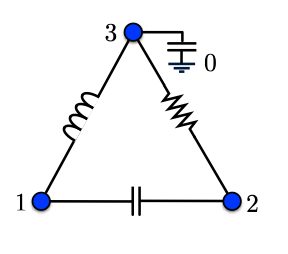
\includegraphics[scale=1]{figs/pn1}
\caption{\label{fig:pn1}sds}
\end{figure}

\end{example}
\begin{figure}
\centering
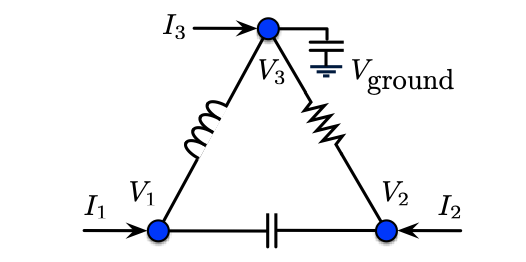
\includegraphics[scale=1]{figs/pn2}
\caption{\label{fig:pn2}sds}
\end{figure}
The basic physical variables are the voltages and currents. On each node we have a potential and a current injection and on each edge we have voltage and current flows. The voltage is a complex number $V=Ee^{i\theta}$ with voltage magnitue and voltage angles.  In Figure \ref{fig:pn2} we see the three external injections $I_1,I_2,I_3$, the three voltage potentials $V_1,V_2,V_3$ and the reference $V_{ground}=0V$. The fundamental equations describing an AC circuit are 
\begin{itemize}
\item Ohm's law  $I_{i\rightarrow j}=\frac{1}{Z_{ij}}(V_i-V_j)$
\item Kirchhoffs current law: $I_i+\sum_j I_{j\rightarrow i}=0$
\item current balance equations $I_i=-\sum_jI_{j\rightarrow i}=\sum_j \frac{1}{Z_{ij}}(V_i-V_j)=\sum_j Y_{ij}V_j$ or $I=Y\cdot V$
\item complex power $S=V_i\bar{I}_i=P+iQ$
\end{itemize}

The power balance equations are formed by setting power injection equal to the sum of the power flows. This leads to
$S_i=V_i\bar{I}_i=\sum_j V_i\bar{Y}_{ij}\bar{V}_j$. Inserting the polar form for $V$ and separating by real and imaginary part we get the power flow equation.
\begin{definition}
Let $G=(V,E)$ be a graph representing the power grid. On each node $i\in V$ a complex voltage $E_ie^{i\theta_i}$ and a complex power $S_i=P_i+iQ_i$ is defined. The AC Power Flow balance equations are given by 
\begin{align}
P_i&=\sum_j B_{ij}E_iE_j\sin{\theta_i-\theta_j}+G_{ij}E_iE_j\cos{\theta_i-\theta_j}\forall i,j\in V\\
Q_i&=\sum_j- B_{ij}E_iE_j\cos{\theta_i-\theta_j}+G_{ij}E_iE_j\sin{\theta_i-\theta_j} \forall i,j\in V
\end{align}

\end{definition}
The power flow equations are a set of $2*N$ real equations, where $N$ is the number of buses on $2*N$ complex variables, which are $4*N$ real variables. This means that we have more variables than equations. However typical buses are modelled as either loads or synchronous generators. Loads have given active power and reactive power and generators have given constant power and voltage magnitude meaning we distiguish between $PQ$ buses and $PV$ buses. There is also the notion of a slack bus where $E$ and $\theta$ are specified. 
\subsection{Physical Units}
Active power (P) is measured in Watt (W) which in SI units is $\frac{kg \;m^2}{s^3}\frac{J}{s}$. Complex Power(S), measured in the same SI units,  is  called volt-ampere and can be a complex number $S=P+iQ$ and $Q$ is the reactive power which is such that $iQ$ is measured in volt-ampere and therefore $Q$ is measuerd in volt-ampere reactive (VAR). Reactive power exists in an AC circuit when the current and voltage are not in phase. The term VAR was proposed by the Romanian electrical engineer Constantin Budeanu and introduced in 1930 by the IEC in Stockholm, which has adopted it as the unit for reactive power. Special instruments called varmeters are available to measure the reactive power in a circuit. Voltage is measured in Volt which is $\frac{kg\; m^2}{As^3}$ in SI units. Current is measured in Ampere $A$,  which means that if we multiply Volt with Ampere we get Watt. The unit of impedance is Ohm which is $\frac{V}{A}=\frac{kg\; m^2}{A^2s^3}$.



\section{The Power Flow Problem}
Roughly speaking, by solving “the power flow problem”, we mean finding the complex voltages for all the buses of the power system when the complex power injections are given such that the power injections and the voltages satisfy the power flow equations. However, there are several considerations:
\subsubsection*{Existence of solutions}
In general we cannot specify all the complex power injections independently, as can be seen from the following two examples:
\begin{itemize}
\item  Consider the case where all the transmission lines are lossless (i.e. $Y$ is a diagonal matrix). Then by the conservation of power, we get that
\[\sum P_i=0,\]
which puts a constraint on the power injection vector.

\item  Consider the case where the power system consists of two buses connected by a short transmission line with admittance $ g + ib$. Then the admittance matrix is
\[\begin{bmatrix} g+ib & -g-ib\\-g-ib & g+ib\end{bmatrix}\]
and the power flow equations are
\begin{align}
P_1 &= g|V_1|^2 + |V_1||V_2|(-g \cos{\theta_2} + b \sin{\theta_2}),\\ P_2 &= g|V_2|^2 + |V_1||V_2|(-g \cos{\theta_2} -b \sin{\theta_2}),\\ 
Q_1 &= -b|V_1|^2 + |V_1||V_2|(g \sin{\theta_2} + b \cos{\theta_2}),\\ Q_2 &= -b|V_2|^2 + |V_1||V_2|(-g \sin{\theta_2} + b \cos{\theta_2}),
\end{align}
and so
\begin{align}
P_1 + P_2 = g(|V_1|^2 + |V_2|^2 -2|V_1||V_2| \cos{\theta_2}) = g|V_1 -V_2|^2,\\
Q_1 + Q_2 = -b(|V_1|^2 + |V_2|^2 - 2b|V_1||V_2| \cos{\theta_2}) = -b|V_1 -V_2|^2,
\end{align} (these two equalities can also be obtained by the conservation of complex
power), which imply that
\[b(P_1 +P_2)+g(Q_1 +Q_2)=0.\]
These two examples suggest that there is a constraint imposed on the power injections by the need to balance complex power in steady-state operation.
\end{itemize}
\subsubsection*{Uniqueness of solution}
The solution in general is not unique: If the complex voltages $V\in\mathbb{C}^N$ and the complex power injections $S\in\mathbb{C}^N$ satisfy the power flow equations, then $e^{j\theta_0} V$ and $S$ will also satisfy the power flow equations for any $\theta_0\in\mathbb{R}$. This means that we need to fix the voltage phase angle at a certain bus.


\begin{remark}For transmission networks, it is reasonable to model loads as constant power loads, meaning that the complex power consumed by the loads are not affected by the voltages imposed on the loads. This is partly related to the fact that in transmission networks, loads are usually connected to the network via substations, in which there are voltage regulators (transformers with variable voltage gains) to keep the voltages on the secondary side roughly constant regardless of the voltages on the primary side.
On the other hand, for buses with bulk generators connected it is more reasonable to specify their real power injections and voltage magnitudes (this is due
to how the bulk generators are operated, which we will not talk about in detail in this course); the reactive power injections will then be determined after the complex voltages are solved.
\end{remark}

There are three types of buses:
\begin{enumerate}
\item  A slack bus or swing bus, at which the voltage phase angle is zero and the
voltage magnitude is given. In other words, $V_1 = |V_1|$ is specified. The slack bus is placed at a generator bus and is usually bus 1.
\item PV buses or voltage-controlled buses, at which the real power injections and the voltage magnitudes are specified. These buses are usually buses with bulk generators connected.
Suppose bus $i$ is a PV bus connected to generators injecting real power $P_{G_i}$ and loads consuming real power $P_{D_i}$, then the net real power injection at bus i is given by $P_i = P_{G_i} - P_{D_i}$.
Without loss of generality we assume that the PV buses are bus 2 to bus M.
\item PQ buses or load buses, at which the real and reactive power injections are specified. These buses are usually the load buses.
Suppose bus $i$ is a PQ bus connected to loads consuming real power $P_{D_i}$ and reactive power $Q_{D_i}$, then the net real and reactive complex power injections at bus $i$ are given by $P_i = -P_{D_i}$, $Q_i = -Q_{D_i}$.
\end{enumerate}


The power flow problem is to find the following $2N - M - 1$ real quantities 
\[\theta_2,...,\theta_M,|V_M+1|,\theta_{M+1},|V_{M+2}|,\theta_{M+2},...,|V_N|,\theta_N\]

from the following $2N - M - 1$ power flow equations
\begin{align}
P_i&=\sum_{k=1}^N |V_i||V_k|(G_{ik}\cos{(\theta_i-\theta_k)}+B_{ij}\sin{(\theta_i-\theta_k)}, i=2,\dots,N\\
Q_i &=\sum_{k=1}^N|V_i||V_k|(G_{ik}\sin{(\theta_i-\theta_k)}-B_{ik}\cos{(\theta_i-\theta_k)}), i=M+1,\dots,N. 
\end{align}

given the following specified quantities
\[|V_1|,\theta_1 = 0,P_2,|V_2|,...,P_M,|V_M|,P_{M+1},Q_{M+1},...P_N,Q_N.\]


 After the $2N - M - 1$ unknown quantities are found, the complex power injection at the slack bus and the reactive power injections at the PV buses are calculated by
\begin{align}
P_1 &=\sum_{k=1}^N |V_1||V_k|(G_{1k}\cos{\theta_k} -B_{1k}\sin{\theta_k}),\\
Q_i &=\sum_{k=1}^N|V_i| |V_k| (G_{ik}\sin{(\theta_i-\theta_k)}-B_{ik}\cos{(\theta_i-\theta_k)}), i=1,\dots,M.
\end{align}
The real and reactive power generated by generators connected to the slack bus are $P_{G_1} = P_1 +P_{D_1}$ and $Q_{G_1} = Q_1 +Q_{D_1}$, where $P_{D_1}$ and $Q_{D_1}$ are the real and reactive power consumption of the load connected to the slack bus. For PV bus $i$, the reactive power generated by generators connected to it is $Q_{G_i} = Q_i + Q_{D_i}$, where $Q_{D_i}$ is the reactive power consumption of the load connected to bus $i$. Moreover, after all the voltages are found, we can then calculate the complex powers and currents that flow through the transmission links, to check if operational constraints (e.g. thermal limits) are satisfied.


\begin{remark}The slack bus plays two roles: (1) to serve as a reference of the voltage phase angles, (2) to achieve power balance of the whole system by not specifying its power injections. Then, since the complex power injection of the slack bus is not predetermined, we will need generators connected to the slack bus so that its complex power injection is adjustable. For a PV bus $i$, usually the reactive power produced by the generators $Q_{G_i}$ must be constrained within a certain range such as $Q_{min} \leq Q_{G_i} \leq Q_{max}$. After solving
the power flow problem and evaluating the resulting reactive power generation $Q_{G_i}$, if it exceeds one of the limits then $Q_{G_i}$ will be set to that limit and bus $i$ will be re-classified as a PQ bus with $|V_i|$ to be determined. The updated power flow equations are then resolved for the unknown quantities.

\end{remark}
The core of solving the power flow problem is solving the $2N - M - 1$ nonlinear power flow equations. These nonlinear equations may have no, one unique, or multiple solutions. The following subsection introduces numerical methods for solving the nonlinear power flow equations.


\subsection{Numerical Solutions}
Solution Methods that can be used to solve the nonlinear system of equation called the power flow equations are methods that do not require the computation of the Jacobian matrix of the nonlinearity (Jacobi's method and Gauss-Seidel’s method), and methods that require the computation of the Jacobian matrix  (Newton’s method and variants)
\subsubsection*{Gauss-Seidel}
This is one of many techniques for solving the nonlinear power flow problem. 
It got the name from an iteration to solve a linear system of the form 
$$
Ax=b$$

The idea for the Gauss-Seidel iteration for this linear system is by splitting $A$ into three matrices $L$ the matrix with the entries of $A$ below or left of the diagonal and zero otherwise, $D$ the diagonal of $A$ and $R$ the entries right of the diagonal and zero otherwise such that
$$
A=L+D+R$$

from that we iterate by considering the following equation

$$
(L+D)x=-Rx+b
$$
giving the iteration 
$$
x^{k+1}=(L+D)^{-1}(-Rx^k+b)
$$
The theory in numerical linear algebra on this iteration scheme and the convergence criteria can be found anywhere in numerical linear algebra textbooks. 


The question now is how can we use this on a nonlinera system of equations. The power flow equation can be written in complex notation as
\[S_i=P_i+iQ_i=E_i\sum Y^*_{ij}E_je^{i(\theta_i-\theta_j)}=V_i\sum Y^*_{ij}V^*_j\]

where $Y_{ij}=G_{ij}+iB_{ij}$

which can be rewritten as

$$
\frac{S_i}{V_i}=\sum Y_{ij}^*V_j^*
$$

By first taking the complex conjugate this can be interpreted as a linear equation with a right hand side still depending on $V$ meaning we have

$$YV=b(V)$$
where $Y$ is the matrix with entries $Y_{ij}$ and $V$ is the vector with entries $V_i$ and $b(V)_i=S^*_i/V^*_i$

Straightforward Gauss-Seidel on this gives us the following iteration
\begin{align}
V_1^{k+1}&=Y_{11}^{-1}(-\sum_{i=2}^{n}Y_{1i}V^k_i+b(V^k)_1)\\
&=Y_{11}^{-1}(-\sum_{i=2}^{n}Y_{1i}V^k_i+\frac{S_1^*}{V_1^*})\\
\end{align}

One can then further see that we get the next entries of the vector $V^{k+1}$ by the following 

$$
V_j^{k+1}=Y_{jj}^{-1}(-\sum_{i=1}^{j-1} Y_{ji}V_i^{k+1}-\sum_{i=j+1}^n Y_{ji}V_i^{k+1}+\frac{S_j^*}{V_j^*})
$$

It should be pointed out that this solution technique, while straightforward to use and easy to understand, has a tendency to use a lot of computation, particularly for large problems. It is also quite capable of converging to incorrect solutions (that is a problem with nonlinear systems). As with other iterative techniques, it is often difficult to tell when the correct solution has been reached. Despite these shortcomings, Gauss–Seidel can be used to get a good feel for power flow problems without excessive numerical analysis baggage.


Suppose we have an initial estimate (ok: guess) for network voltages. This expressions gives a better estimate of $V_i$ than we started with. The solution to the set of nonlinear equations consists of carrying out this expression, repeatedly, for all of the buses of the network.


For generator buses, usually the real power and terminal voltage magnitude are specified. At each time step it is necessary to come out with a terminal voltage of specified magnitude: voltage phase angle and reactive power $Q$ are the unknowns. One way of handling this situation is to:
\begin{enumerate}

\item Generate an estimate for reactive power Q, then
\item Use the equations to generate an estimate for terminal voltage, and finally,
\item Holding voltage phase angle constant, adjust magnitude to the constraint.

\end{enumerate}
At any point in the iteration, reactive power is:
\[Q_i=\textsl{im}{(V_i\sum Y^*_{ij}V_j^*)}\]

It should be noted that there are other ways of doing this calculation. Generally they are more work to set up but often converge more quickly. Newton’s method and variations are good examples.

For buses loaded by constant impedance, it is sufficient to lump the load impedance into the network. That is, the load admittance goes directly in parallel with the driving point admittance at the node in question.
These three bus constraint types, generator, load and constant impedance are sufficient for handling most problems of practical importance.


\section{Dynamic Model for Transient Stability}
The power flow is used to determine a quasi steady-state operating condition for a power system. Dynamics simulations are used to determine whether following a contingency the power system returns to a steady-state operating point or not. If returning to a steady state is not garantueed, the system can  become instable. The ideal situation is that the system starts in a steady-state, and hopefully returns to a new steady-state value.
In order to operate as an interconnected system, all of the generators (and other synchronous machines) must remain in synchronism, with one another. Synchronism requires that (for two pole machines) the rotors turn at the same speed. Loss of synchronism results in a condition in which no net power can be transferred between the machines. A system is said to be transiently unstable if following a disturbance one or more of the generators lose synchronism.
In order to study the transient response of a power system we need to develop models for the generator valid during the transient time frame of several seconds following a system disturbance.
We need to develop both electrical and mechanical models for the generators.
The simplest generator model, known as the classical model, treats the generator as a voltage source behind the direct-axis transient reactance; the voltage magnitude is fixed, but its angle changes according to the mechanical dynamics 
resulting in the following type of ordinary differential equation as described by Machowski et al.
(2008)
\[m_i\ddot{\delta_i}+d_i\dot{\delta}_i=P_i^m-\sum k_{ij}\sin{\delta_i-\delta_j}\]
where $\delta_i$ is the phase angle of bus $i$, $m_i$ and $d_i$ are the inertia and damping coefficient
respectively, $p_i^m$
is the power load at bus $i$ and $k_{ij} = |V_i||V_j|B_{ij}$, where $V_i$ is the voltage of bus $i$, and $B_{ij}$ is the susceptance of the
line $(i, j)$. By convention
we will define injected power to have a positive sign, and power load to have a negative
sign. 

In vector notation the system can be written as

\[M\ddot{\delta}+D\dot{\delta}=f(\delta)\]
and in first order form 

\[\begin{bmatrix} \dot{\omega}\\ \dot{\delta}\end{bmatrix}=
\begin{bmatrix}-M^{-1}D & 0 \\ I & 0\end{bmatrix}\begin{bmatrix}\omega \\ \delta\end{bmatrix}+\begin{bmatrix}f(\delta)\\0\end{bmatrix}\]

%Lets go back to the model of a bus by 
%
%\[m_i\ddot{\delta_i}+d_i\dot{\delta}_i=P_i^m-\sum k_{ij}\sin{\delta_i-\delta_j}\]

We will assume that generator buses are modeled like this and possible other nodes as well, but we will also introduce nodes which satisfy a first order equation leading to the following model

\begin{align}
m_i\ddot{\delta_i}+d_i\dot{\delta}_i&=P_i^m-\sum k_{ij}\sin{\delta_i-\delta_j}\quad i\in V_p\\
d_i\dot{\delta}_i&=P_i^m-\sum k_{ij}\sin{\delta_i-\delta_j}\quad i\in      V_c
\end{align}


This system of equation can be linearized
\begin{align*}
m_i\ddot{\delta_i}+d_i\dot{\delta}_i&=P_i^m-\sum k_{ij}
\cos{(\delta^*_i-\delta^*_j)}(\delta_i-\delta_j)\quad i\in V_p\\
d_i\dot{\delta}_i&=P_i^m-\sum k_{ij}\cos{(\delta^*_i-\delta^*_j)}(\delta_i-\delta_j)\quad i\in V_c
\end{align*}

and then the right hand side of this system is equal to $L\delta$ with $L$ being

\[L=\left\{\begin{matrix}-k_{ij}\cos{(\delta_i^*-
\delta^*_j)} &\mbox{if } i\neq j\\
\sum_{i\neq ji}k_{ij}\cos{(\delta_i^*-
\delta^*_j)}&\mbox{ else}\end{matrix}\right.\]
which is the Laplacian matrix for small perturbations around an operating point.
The linearised power system model is then given
as:

\[M\ddot{\delta}+D\dot{\delta} =P^m-L\delta\]

The topological properties of the network are encoded in the Laplacian matrix $L$.
$M$ and $D$ are diagonal matrices which describe the machine parameters at each node
in the system. Typically M is a singular diagonal
matrix. As we are mostly interested in the influence of the topology and
machine parameters, we will focus on the free response system by setting $P^m = 0$.

The solution to the system $M\ddot{\delta}+D\dot{\delta}+L\delta=0$ is given by 

\[\delta(t)=\sum_{k=1}^{2N} \gamma_k\phi_k\exp{\lambda_k t}\]

where the $\gamma$ come from the initial value and $\lambda$ and $\phi$ are solutions of the quadratic eigenvalue problem:

\[(\lambda^2M+\lambda D+L)\phi=0\]
\subsection*{Quadratic Eigenvalue Problem}
The quadratic eigenvalue problem is directly related to the eigenvalue problem,
with the differences being the additional matrices $M$ and $D$ and supplementary
quadratic and linear eigenvalue terms. Even when the matrices are of size $n$ by $n$, the
quadratic nature results in $2n$ eigenpairs. This can be understood as a result of the
positive and negative solutions of a square root. From a theoretical point of view,
the following properties can be found in a QEP:
\begin{enumerate}
\item  $M$ is non singular - $2n$ finite eigenvalues
\item $M$, $D$, $L$ are real matrices - eigenvalues are either real or come in complex conjugate
pairs
\item $M$ hermitian and positive definite, $D$ and $L$ positive semi definite - The real
parts of the eigenvalues are non positive
\end{enumerate}
When $M$ is singular, there will be infinite eigenvalues. As $M$ is a diagonal matrix
with zero entries for the load nodes, there are infinite eigenvalues. 



%
\end{document}